% Mustafa Alparslan
%X: book 1
%Y: part 2
%ZZZ: page 355.

\documentclass[11pt]{amsbook}

\usepackage{../HBSuerDemir}	% ------------------------

\usepackage{wrapfig}

\begin{document}

% ++++++++++++++++++++++++++++++++++++++
\hPage{b1p2/355}
% ++++++++++++++++++++++++++++++++++++++

is called the \textit{average value} of $f(x)$ on $(a, b)$ with respect to $x$.

\centerline{\textbf{\underline{Geometric Interpretation of the MVT for Integral}}:}

\begin{wrapfigure}{R}{0.45\textwidth} 
\centering
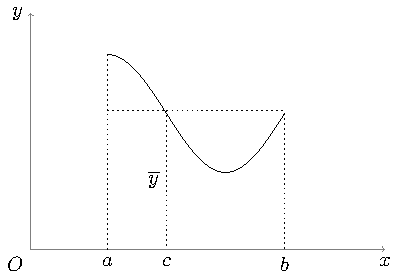
\includegraphics[width=0.40\textwidth]{images/b1p2-355-fig01.pdf}
\label{fig:b1p2-355-fig01.pdf}
\end{wrapfigure}

The definite integral  \footnote{Image with wrapfigure. Images were drawn with tikzpicture and can be found in the imageSources folder.}

\[
\int_{a}^{b} f(x) dx
\]

is equal to the length of interval times the average value of the function. 

In particular when $f(x) > 0$, the area given by the integral is equal to the area of the rectange with base $b-a$ and altitude $\overline{y} = f(c)$.

\begin{exmp}
Find the average value of  $ y = \sqrt{a^2 - x^2 }$ in $(0,\, a)$ with respect to \textit{x}.
\end{exmp}

 \begin{wrapfigure}{R}{0.35 \textwidth}
 \centering
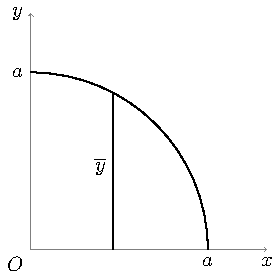
\includegraphics[width=0.30\textwidth]{images/b1p2-355-fig02.pdf} 
\label{fig:b1p2-355-fig02}
\end{wrapfigure}

\textbf{Solution} \quad
\( 
\int_{0}^{b} \sqrt{ a^2 - x^2 } = \frac{\pi}{4} \, a^2
\)
since it is the area of the quarter of the circle with radius $a$.

The length of the interval being $a$, we have

\[ 
\overline{y} 
= \frac{\pi}{4} \, a^2 / a 
= \frac{\pi}{4} \, a \quad (<  \, a).
\]

When $f(x)$ is interpreted as a physical quantity such as density, energy, force, etc. $\overline{y}$ will mean averages of these quantities. 

\begin{thm} (F.T. of Calculus). If $f(x) \quad C(a, b)$ then   $\int_{a}^{x}\ f(t)\, dt$ is differentiable function, and
\[
\frac{d}{dx} \quad 
\int_{a}^{x} f(t) dt 
\: = \: 
f(x)
\]

\end{thm}
% =======================================================
\end{document}  
